\documentclass[../piano-di-qualifica.tex]{subfiles}

\begin{document}
In questa sezione vengono resi noti i risultati dei test relativi al periodo di revisione dei documenti e requisiti, mediante l'utilizzo delle metriche descritte nelle sezioni precedenti.
I risultati possono coincidere o meno con i valori desiderati dal gruppo, nel caso non coincidessero verrà fatta un ulteriore analisi per il miglioramento visibile nel punto §7.

\subsection{Primo periodo (RR)}
\label{sub:primo_periodo}
Durante questo periodo è stata sottoposta ad una precisa attività di verifica tutta la documentazione da presentare in ingresso in sede di Revisione dei Requisiti.
I verificatori inizialmente hanno effettuato l'analisi utilizzando la tecnica di \glossario{Walkthrough} che ha portato ad una serie di errori frequenti consultabili nella sezione appendice §C del documento.
Successivamente dopo questa prima fase, i verificatori mediante la tecnica dell'\glossario{Inspection} hanno analizzato i documenti in modo più mirato ricavando errori di diverso genere che non verranno trattati in quanto si trattano di piccolezze già facilmente risolte.

\subsubsection{Esiti verifiche sui documenti}
\label{sub:esiti_verifiche_sui_documenti}
Sui documenti sono state utilizzate le metriche per:
    \begin{itemize}
        \item \textbf{Indice di Gulpease};
        \item \textbf{Correttezza lessicale/ortografica}.
    \end{itemize}
Per evitare risultati errati nel calcole dell'Indice di Gulpease si è deciso di non tenere in considerazione:
    \begin{itemize}
        \item Il frontespizio di ogni documento;
        \item Le tabelle presenti nei documenti;
        \item Il diario delle modifiche all'interno di ogni documento.
    \end{itemize}
Per quanto riguarda la correttezza lessicale/ortografica, gli errori trovati non verranno classificati ma semplicemente conteggiati uniformemente includendo anche errori derivati dal mancato rispetto delle convenzioni scritte nelle \textsc{Norme di Progetto v1.0.0}.
\\ Per ogni metrica di ogni documento verrà inoltre inserito l'esito dell'analisi che può avere risultato soddisfacente o non.

\paragraph{Norme di Progetto}
\label{sub:norme_di_progetto}
Pur essendo le \textsc{Norme di Progetto v1.0.0} un documento abbastanza corposo e ricco di pagine di spiegazione, il numero di errori trovati non è molto alto ed è progressivamente calato in base alle versioni del documento dopo ogni fase di verifica delle modifiche, grazie anche a una buona verifica da parte dei Verificatori e di tutto il team.
Il documento ha ottenuto un punteggio di circa 70 per quanto riguarda l'indice di Gulpease, il che è perfettamente in linea con l'obiettivo prefissato.

\rowcolors{2}{white!80!lightgray!90}{white}
\renewcommand{\arraystretch}{2} % allarga le righe con dello spazio sotto e sopra
\begin{longtable}[H]{>{\centering\bfseries}m{6cm} >{\centering}m{2cm} >{\centering}m{2.5cm} >{\centering}m{2.5cm} >{\centering\arraybackslash}m{2.5cm}}  
  \rowcolor{lightgray}
  {\textbf{Documento}} & {\textbf{Risultato indice}} & {\textbf{Errori presenti}} & {\textbf{Esito indice}} & {\textbf{Esito errori}}  \\
  \endfirsthead%
  \rowcolor{lightgray}
  {\textbf{Documento}} & {\textbf{Risultato indice}} & {\textbf{Errori presenti}} & {\textbf{Esito indice}} & {\textbf{Esito errori}}  \\
  \endhead%
  \textbf{Norme di Progetto v1.0.0} &  70                & 0               & Soddisfatto & Soddisfatto \\
  \caption{Risultati metriche per le Norme di Progetto v1.0.0}
  \label{tab:my-table}
\end{longtable}

    \begin{figure}[H]
        \centering
        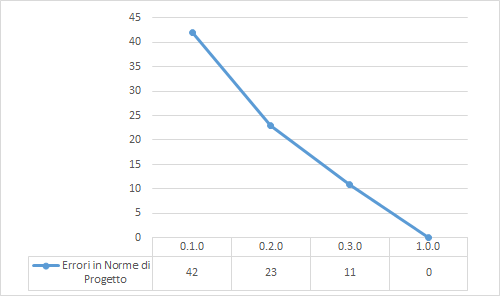
\includegraphics[width=10cm]{img/erroriNorme.png}
        \label{fig:scice_documenti}
        \caption{Grafico errori per \textsc{Norme Di Progetto v1.0.0}}
    \end{figure}

\paragraph{Studio di Fattibilità}
\label{sub:studio_di_fattibilita}
Essendo lo \textsc{Studio di Fattibilità v1.0.0} uno dei primi documenti redatti dal gruppo, il numero di errori è risultato alto rispetto al contenuto soprattutto per errori di dimenticanza nel rispettare quanto scritto nelle \textsc{Norme di Progetto v1.0.0}.
In questo documento sono state fatte 2 sole fasi di verifica in quanto il documento aveva contenuti più ristretti rispetto agli altri documenti e dopo la seconda verifica non vi sono stati aggiunti ulteriori contenuti.
Il risultato dell'indice di Gulpease è di 68 che soddisfa il valore accettabile dell'obiettivo.

\rowcolors{2}{white!80!lightgray!90}{white}
\renewcommand{\arraystretch}{2} % allarga le righe con dello spazio sotto e sopra
\begin{longtable}[H]{>{\centering\bfseries}m{6cm} >{\centering}m{2cm} >{\centering}m{2.5cm} >{\centering}m{2.5cm} >{\centering\arraybackslash}m{2.5cm}}  
  \rowcolor{lightgray}
  {\textbf{Documento}} & {\textbf{Risultato indice}} & {\textbf{Errori presenti}} & {\textbf{Esito indice}} & {\textbf{Esito errori}}  \\
  \endfirsthead%
  \rowcolor{lightgray}
  {\textbf{Documento}} & {\textbf{Risultato indice}} & {\textbf{Errori presenti}} & {\textbf{Esito indice}} & {\textbf{Esito errori}}  \\
  \endhead%
  \textbf{Studio di Fattibilità v1.0.0} & 68                 & 0               & Soddisfatto & Soddisfatto \\
  \caption{Risultati metriche per lo Studio di Fattibilità v1.0.0}
  \label{tab:my-table}
\end{longtable}

    \begin{figure}[H]
        \centering
        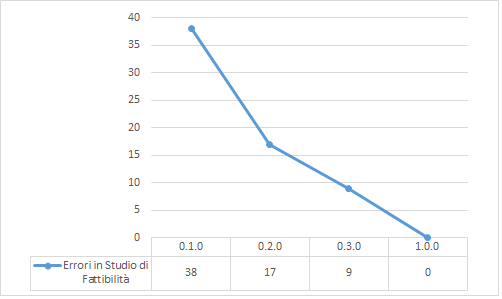
\includegraphics[width=10cm]{img/erroriStudio.png}
        \label{fig:scice_documenti}
        \caption{Grafico errori per \textsc{Studio di Fattibilità v1.0.0}}
    \end{figure}

\paragraph{Piano di Qualifica}
\label{sub:piano_di_qualifica}
Il \textsc{Piano di Qualifica v1.0.0} ha presentato molti errori durante la sua realizzazione soprattutto nelle fasi di verifica in cui sono state realizzate le versioni 0.1.0 e 0.3.0 in quanto in quei periodi sono stati redatti gran parte dei contenuti del piano.
Essendo un documento ricco di sezioni e contenuti si è reso necessario effettuare 4 fasi di verifica per il documento.
L'indice di Gulpease, il cui risultato è 73, del documento rientra nel range definito tra 65 e 75.

\rowcolors{2}{white!80!lightgray!90}{white}
\renewcommand{\arraystretch}{2} % allarga le righe con dello spazio sotto e sopra
\begin{longtable}[H]{>{\centering\bfseries}m{6cm} >{\centering}m{2cm} >{\centering}m{2.5cm} >{\centering}m{2.5cm} >{\centering\arraybackslash}m{2.5cm}}  
  \rowcolor{lightgray}
  {\textbf{Documento}} & {\textbf{Risultato indice}} & {\textbf{Errori presenti}} & {\textbf{Esito indice}} & {\textbf{Esito errori}}  \\
  \endfirsthead%
  \rowcolor{lightgray}
  {\textbf{Documento}} & {\textbf{Risultato indice}} & {\textbf{Errori presenti}} & {\textbf{Esito indice}} & {\textbf{Esito errori}}  \\
  \endhead%
  \textbf{Piano di Qualifica v1.0.0} &  73               & 0               & Soddisfatto & Soddisfatto \\
  \caption{Risultati metriche per il Piano di Qualifica v1.0.0}
  \label{tab:my-table}
\end{longtable}

\begin{figure}[H]
    \centering
    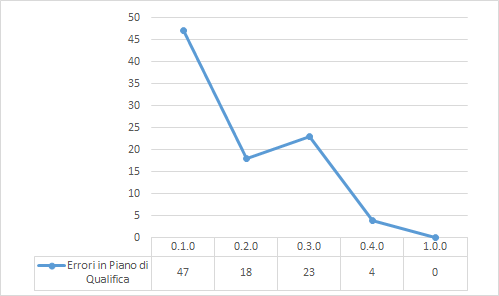
\includegraphics[width=10cm]{img/erroriPdQ.png}
    \label{fig:scice_documenti}
    \caption{Grafico errori per \textsc{Piano di Qualifica v1.0.0}}
\end{figure}

\paragraph{Piano di Progetto}
\label{sub:piano_di_progetto}
Il \textsc{Piano di Progetto v1.0.0} ha presentato parecchi errori inizialmente così come il \textsc{Piano di Qualifica v1.0.0} ma dopo ogni verifica il numero di errori è sceso in modo quasi lineare fino a raggiungere l'obiettivo di 0 errori prefissato.
L'indice di Gulpease rilevato, del documento è 75 che eguaglia il valore desiderabile dell'obiettivo.

\rowcolors{2}{white!80!lightgray!90}{white}
\renewcommand{\arraystretch}{2} % allarga le righe con dello spazio sotto e sopra
\begin{longtable}[H]{>{\centering\bfseries}m{6cm} >{\centering}m{2cm} >{\centering}m{2.5cm} >{\centering}m{2.5cm} >{\centering\arraybackslash}m{2.5cm}}  
  \rowcolor{lightgray}
  {\textbf{Documento}} & {\textbf{Risultato indice}} & {\textbf{Errori presenti}} & {\textbf{Esito indice}} & {\textbf{Esito errori}}  \\
  \endfirsthead%
  \rowcolor{lightgray}
  {\textbf{Documento}} & {\textbf{Risultato indice}} & {\textbf{Errori presenti}} & {\textbf{Esito indice}} & {\textbf{Esito errori}}  \\
  \endhead%
  \textbf{Piano di Progetto v1.0.0} & 75                 & 0               & Soddisfatto & Soddisfatto \\
  \caption{Risultati metriche per il Piano di Progetto v1.0.0}
  \label{tab:my-table}
\end{longtable}

\begin{figure}[H]
    \centering
    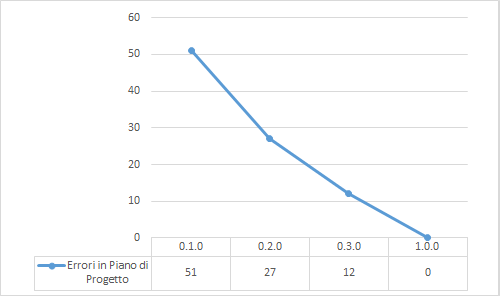
\includegraphics[width=10cm]{img/erroriPdP.png}
    \label{fig:scice_documenti}
    \caption{Grafico errori per \textsc{Piano di Progetto v1.0.0}}
\end{figure}

\paragraph{Analisi dei Requisiti}
\label{sub:analisi_dei_requisiti}
Come per le \textsc{Norme di Progetto v1.0.0} essendo anche l'\textsc{Analisi dei Requisiti v1.0.0} un documento abbastanza corposo il numero di errori rilevati durante le verifiche è stato elevato ma non eccessivo, inoltre si nota che nella fase di verifica che ha portato alla creazione della versione 0.3.0 il numero di errori è drasticamente calato. 
L'indice di Gulpease, essendo 73, rientra nel range desiderato per l'obiettivo.

\rowcolors{2}{white!80!lightgray!90}{white}
\renewcommand{\arraystretch}{2} % allarga le righe con dello spazio sotto e sopra
\begin{longtable}[H]{>{\centering\bfseries}m{6cm} >{\centering}m{2cm} >{\centering}m{2.5cm} >{\centering}m{2.5cm} >{\centering\arraybackslash}m{2.5cm}}  
  \rowcolor{lightgray}
  {\textbf{Documento}} & {\textbf{Risultato indice}} & {\textbf{Errori presenti}} & {\textbf{Esito indice}} & {\textbf{Esito errori}}  \\
  \endfirsthead%
  \rowcolor{lightgray}
  {\textbf{Documento}} & {\textbf{Risultato indice}} & {\textbf{Errori presenti}} & {\textbf{Esito indice}} & {\textbf{Esito errori}}  \\
  \endhead%
  \textbf{Analisi dei Requisiti v1.0.0} & 73                 & 0               & Soddisfatto & Soddisfatto \\
  \caption{Risultati metriche per l'Analisi dei Requisiti v1.0.0}
  \label{tab:my-table}
\end{longtable}

    \begin{figure}[H]
        \centering
        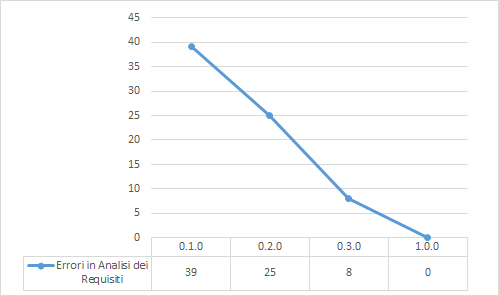
\includegraphics[width=10cm]{img/erroriAnalisi.png}
        \label{fig:scice_documenti}
        \caption{Grafico errori per \textsc{Analisi dei Requisiti v1.0.0}}
    \end{figure}

\paragraph{Glossario}
\label{sub:glossario}
Essendo il \textsc{Glossario v1.0.0} un documento abbastanza semplice e con lo scopo di informare il lettore sul significato di termini particolari, si è deciso di effettuare una sola fase di verifica finale.     
L'indice di Gulpease di questo documento è 65, che risulta essere al limite col valore accettabile, ma soddisfa comunque l'obiettivo.

\rowcolors{2}{white!80!lightgray!90}{white}
\renewcommand{\arraystretch}{2} % allarga le righe con dello spazio sotto e sopra
\begin{longtable}[H]{>{\centering\bfseries}m{6cm} >{\centering}m{2cm} >{\centering}m{2.5cm} >{\centering}m{2.5cm} >{\centering\arraybackslash}m{2.5cm}}  
  \rowcolor{lightgray}
  {\textbf{Documento}} & {\textbf{Risultato indice}} & {\textbf{Errori presenti}} & {\textbf{Esito indice}} & {\textbf{Esito errori}}  \\
  \endfirsthead%
  \rowcolor{lightgray}
  {\textbf{Documento}} & {\textbf{Risultato indice}} & {\textbf{Errori presenti}} & {\textbf{Esito indice}} & {\textbf{Esito errori}}  \\
  \endhead%
  \textbf{Glossario v1.0.0} & 65                 & 0               & Soddisfatto & Soddisfatto \\
  \caption{Risultati metriche per il Glossario v1.0.0}
  \label{tab:my-table}
\end{longtable}

\begin{figure}[H]
  \centering
  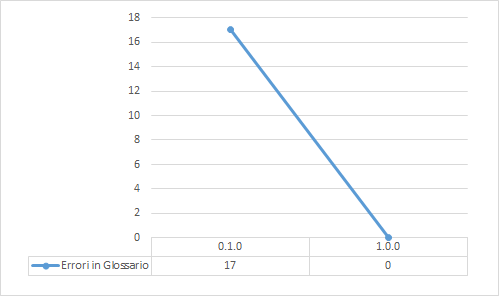
\includegraphics[width=10cm]{img/erroriGlossario.png}
  \label{fig:scice_documenti}
  \caption{Grafico errori per \textsc{Glossario v1.0.0}}
\end{figure}

\subsubsection{Esiti verifiche sui processi}
\label{sub:esiti_verifiche_sui_processi}
In questa sezione vengono visualizzati gli esiti delle metriche prese in considerazione per quanto riguarda i processi produttivi.
Come per i documenti, anche per queste metriche verrà fornito un esito che può essere soddisfacente o meno.

\paragraph{Processo PRC001}
\label{sub:processo_PRC001}

\rowcolors{2}{white!80!lightgray!90}{white}
\renewcommand{\arraystretch}{2} % allarga le righe con dello spazio sotto e sopra
\begin{longtable}[H]{>{\centering\bfseries}m{5cm} >{\centering}m{5cm} >{\centering}m{2.5cm} >{\centering\arraybackslash}m{2.5cm}}  
  \rowcolor{lightgray}
  {\textbf{Obiettivo}} & {\textbf{Metrica}} & {\textbf{Risultato}} & {\textbf{Esito}}  \\
  \endfirsthead%
  \rowcolor{lightgray}
  {\textbf{Obiettivo}} & {\textbf{Metrica}} & {\textbf{Risultato}} & {\textbf{Esito}}  \\
  \endhead%
  \textbf{QoPR001 Rispetto delle scadenze della pianificazione} & MoPR001 Varianza dei tempi & 1.31 & Soddisfatto \\
  \caption{Risultati metrica MoPR001}
  \label{tab:my-table}
\end{longtable}
\textbf{Nota}: il ritardo medio, nel rispetto delle scadenze interne al gruppo, è stato di 1.31 giorni che soddisfa la metrica in quanto non sono stati superati i 2 giorni di media.

\rowcolors{2}{white!80!lightgray!90}{white}
\renewcommand{\arraystretch}{2} % allarga le righe con dello spazio sotto e sopra
\begin{longtable}[H]{>{\centering\bfseries}m{5cm} >{\centering}m{5cm} >{\centering}m{2.5cm} >{\centering\arraybackslash}m{2.5cm}}  
  \rowcolor{lightgray}
  {\textbf{Obiettivo}} & {\textbf{Metrica}} & {\textbf{Risultato}} & {\textbf{Esito}}  \\
  \endfirsthead%
  \rowcolor{lightgray}
  {\textbf{Obiettivo}} & {\textbf{Metrica}} & {\textbf{Risultato}} & {\textbf{Esito}}  \\
  \endhead%
  \textbf{QoPR002 Rispetto del budget istanziato} & MoPR002 Varianza dei costi & +40 & Soddisfatto \\
  \caption{Risultati metrica MoPR002}
  \label{tab:my-table}
\end{longtable}
\textbf{Nota}: la variazione rispetto al preventivo iniziale rientra nel range deciso per la metrica per cui l'obiettivo in questa fase è stato soddisfatto. L'aumento rilevato è: +40 euro;

\rowcolors{2}{white!80!lightgray!90}{white}
\renewcommand{\arraystretch}{2} % allarga le righe con dello spazio sotto e sopra
\begin{longtable}[H]{>{\centering\bfseries}m{5cm} >{\centering}m{5cm} >{\centering}m{2.5cm} >{\centering\arraybackslash}m{2.5cm}}  
  \rowcolor{lightgray}
  {\textbf{Obiettivo}} & {\textbf{Metrica}} & {\textbf{Risultato}} & {\textbf{Esito}}  \\
  \endfirsthead%
  \rowcolor{lightgray}
  {\textbf{Obiettivo}} & {\textbf{Metrica}} & {\textbf{Risultato}} & {\textbf{Esito}}  \\
  \endhead%
  \textbf{QoPR003 Rispetto del ciclo di vita scelto} & MoPR003 Aderenza agli standard & Livello di maturità: 2 Valutazione attributi: L & Non soddisfatto \\
  \caption{Risultati metrica MoPR003}
  \label{tab:my-table}
\end{longtable}
\textbf{Nota}: essendo il progetto ancora nelle fasi iniziali è prevedibile che il livello di maturità desiderato non sia ancora stato soddisfatto in quanto il raggiungimento dell'obiettivo è fissato per la fine del progetto.

\rowcolors{2}{white!80!lightgray!90}{white}
\renewcommand{\arraystretch}{2} % allarga le righe con dello spazio sotto e sopra
\begin{longtable}[H]{>{\centering\bfseries}m{5cm} >{\centering}m{5cm} >{\centering}m{2.5cm} >{\centering\arraybackslash}m{2.5cm}}  
  \rowcolor{lightgray}
  {\textbf{Obiettivo}} & {\textbf{Metrica}} & {\textbf{Risultato}} & {\textbf{Esito}}  \\
  \endfirsthead%
  \rowcolor{lightgray}
  {\textbf{Obiettivo}} & {\textbf{Metrica}} & {\textbf{Risultato}} & {\textbf{Esito}}  \\
  \endhead%
  \textbf{QoPR004 Rispetto dei ruoli e identificazione nei prodotti} & MoPR004 Aderenza ai ruoli & 0 & Soddisfatto \\
  \caption{Risultati metrica MoPR004}
  \label{tab:my-table}
\end{longtable}
\textbf{Nota}: in ogni documento prodotto i ruoli sono stati identificati e rispettati.

\rowcolors{2}{white!80!lightgray!90}{white}
\renewcommand{\arraystretch}{2} % allarga le righe con dello spazio sotto e sopra
\begin{longtable}[H]{>{\centering\bfseries}m{5cm} >{\centering}m{5cm} >{\centering}m{2.5cm} >{\centering\arraybackslash}m{2.5cm}}  
  \rowcolor{lightgray}
  {\textbf{Obiettivo}} & {\textbf{Metrica}} & {\textbf{Risultato}} & {\textbf{Esito}}  \\
  \endfirsthead%
  \rowcolor{lightgray}
  {\textbf{Obiettivo}} & {\textbf{Metrica}} & {\textbf{Risultato}} & {\textbf{Esito}}  \\
  \endhead%
  \textbf{QoPR005 Rispetto del versionamento dei prodotti} & MoPR005 Controllo prodotti & 21.4 & Soddisfatto \\
  \caption{Risultati metrica MoPR005}
  \label{tab:my-table}
\end{longtable}
\textbf{Nota}: essendo la media dei commit nella repository oltre il valore desiderabile (che era 20), l'obiettivo è pienamente soddisfatto.

\paragraph{Processo PRC003}
\label{sub:processo_PRC003}

\rowcolors{2}{white!80!lightgray!90}{white}
\renewcommand{\arraystretch}{2} % allarga le righe con dello spazio sotto e sopra
\begin{longtable}[H]{>{\centering\bfseries}m{5cm} >{\centering}m{5cm} >{\centering}m{2.5cm} >{\centering\arraybackslash}m{2.5cm}}  
  \rowcolor{lightgray}
  {\textbf{Obiettivo}} & {\textbf{Metrica}} & {\textbf{Risultato}} & {\textbf{Esito}}  \\
  \endfirsthead%
  \rowcolor{lightgray}
  {\textbf{Obiettivo}} & {\textbf{Metrica}} & {\textbf{Risultato}} & {\textbf{Esito}}  \\
  \endhead%
  \textbf{QoPR010 Rispetto nella redazione dei documenti} & MoPR011 Analisi documenti & 3 & Soddisfatto \\
  \caption{Risultati metrica MoPR011}
  \label{tab:my-table}
\end{longtable}
\textbf{Nota}: tutti i documenti più corposi e discorsivi sono stati verificati almeno 3 volte, mentre per i documenti più esili di contenuti sono bastate 1 o 2 fasi di verifica. Nonostante tutto il team ritiene l'obiettivo comunque soddisfatto soprattutto per il fatto che non sono stati rilasciati documenti con errori.

\subsubsection{Conclusioni}%
\label{sub:conclusioni}
I dati analizzati esprimono un buon andamento del lavoro svolto dal team che si prefissa come obiettivo quello di continuare a migliorare sotto ogni aspetto relativo alle metriche e agli obiettivi prefissati.
Nei periodi prossimi di realizzazione del progetto il team cercherà di mantenere questi risultati e, se possibile, migliorarli specialmente negli obiettivi più carenti rilevati in questa fase iniziale.

\subsection{Secondo periodo (RP)}
\label{sub:secondo_periodo}
Nella seconda parte del progetto si è attuata una verifica più approfondita sui documenti, correggendo eventuali errori concettuali individuati nella prima fase di Revisione dei Requisiti.
Sono quindi state attuate verifiche e modifiche più specifiche ai documenti, e verifiche sul software, in particolare sul codice scritto per il \glossario{Proof of Concept}.
Come per il primo periodo, gli errori rilevati verranno trattati nella sezione appendice §C del documento.

\subsubsection{Esiti verifiche sui documenti}
\label{sub:esiti_verifiche_sui_documenti}
Sui documenti sono state utilizzate le metriche per:
    \begin{itemize}
        \item \textbf{Indice di Gulpease};
        \item \textbf{Correttezza lessicale/ortografica}.
    \end{itemize}
Per evitare risultati errati nel calcole dell'Indice di Gulpease si è deciso di non tenere in considerazione:
    \begin{itemize}
        \item Il frontespizio di ogni documento;
        \item Le tabelle presenti nei documenti;
        \item Il diario delle modifiche all'interno di ogni documento.
    \end{itemize}
Per quanto riguarda la correttezza lessicale/ortografica, gli errori trovati non verranno classificati ma semplicemente conteggiati uniformemente includendo anche errori derivati dal mancato rispetto delle convenzioni scritte nelle \textsc{Norme di Progetto v2.0.0}.
\\ Per ogni metrica di ogni documento verrà inoltre inserito l'esito dell'analisi che può avere risultato soddisfacente o non.

\paragraph{Norme di Progetto}
\label{sub:norme_di_progetto}

\rowcolors{2}{white!80!lightgray!90}{white}
\renewcommand{\arraystretch}{2} % allarga le righe con dello spazio sotto e sopra
\begin{longtable}[H]{>{\centering\bfseries}m{6cm} >{\centering}m{2cm} >{\centering}m{2.5cm} >{\centering}m{2.5cm} >{\centering\arraybackslash}m{2.5cm}}  
  \rowcolor{lightgray}
  {\textbf{Documento}} & {\textbf{Risultato indice}} & {\textbf{Errori presenti}} & {\textbf{Esito indice}} & {\textbf{Esito errori}}  \\
  \endfirsthead%
  \rowcolor{lightgray}
  {\textbf{Documento}} & {\textbf{Risultato indice}} & {\textbf{Errori presenti}} & {\textbf{Esito indice}} & {\textbf{Esito errori}}  \\
  \endhead%
  \textbf{Norme di Progetto v2.0.0} &                  & 0               & Soddisfatto & Soddisfatto \\
  \caption{Risultati metriche per le Norme di Progetto v2.0.0}
  \label{tab:my-table}
\end{longtable}


\paragraph{Studio di Fattibilità}
\label{sub:studio_di_fattibilita}

\rowcolors{2}{white!80!lightgray!90}{white}
\renewcommand{\arraystretch}{2} % allarga le righe con dello spazio sotto e sopra
\begin{longtable}[H]{>{\centering\bfseries}m{6cm} >{\centering}m{2cm} >{\centering}m{2.5cm} >{\centering}m{2.5cm} >{\centering\arraybackslash}m{2.5cm}}  
  \rowcolor{lightgray}
  {\textbf{Documento}} & {\textbf{Risultato indice}} & {\textbf{Errori presenti}} & {\textbf{Esito indice}} & {\textbf{Esito errori}}  \\
  \endfirsthead%
  \rowcolor{lightgray}
  {\textbf{Documento}} & {\textbf{Risultato indice}} & {\textbf{Errori presenti}} & {\textbf{Esito indice}} & {\textbf{Esito errori}}  \\
  \endhead%
  \textbf{Studio di Fattibilità v2.0.0} &                  & 0               & Soddisfatto & Soddisfatto \\
  \caption{Risultati metriche per lo Studio di Fattibilità v2.0.0}
  \label{tab:my-table}
\end{longtable}


\paragraph{Piano di Qualifica}
\label{sub:piano_di_qualifica}

\rowcolors{2}{white!80!lightgray!90}{white}
\renewcommand{\arraystretch}{2} % allarga le righe con dello spazio sotto e sopra
\begin{longtable}[H]{>{\centering\bfseries}m{6cm} >{\centering}m{2cm} >{\centering}m{2.5cm} >{\centering}m{2.5cm} >{\centering\arraybackslash}m{2.5cm}}  
  \rowcolor{lightgray}
  {\textbf{Documento}} & {\textbf{Risultato indice}} & {\textbf{Errori presenti}} & {\textbf{Esito indice}} & {\textbf{Esito errori}}  \\
  \endfirsthead%
  \rowcolor{lightgray}
  {\textbf{Documento}} & {\textbf{Risultato indice}} & {\textbf{Errori presenti}} & {\textbf{Esito indice}} & {\textbf{Esito errori}}  \\
  \endhead%
  \textbf{Piano di Qualifica v2.0.0} &                 & 0               & Soddisfatto & Soddisfatto \\
  \caption{Risultati metriche per il Piano di Qualifica v2.0.0}
  \label{tab:my-table}
\end{longtable}


\paragraph{Piano di Progetto}
\label{sub:piano_di_progetto}

\rowcolors{2}{white!80!lightgray!90}{white}
\renewcommand{\arraystretch}{2} % allarga le righe con dello spazio sotto e sopra
\begin{longtable}[H]{>{\centering\bfseries}m{6cm} >{\centering}m{2cm} >{\centering}m{2.5cm} >{\centering}m{2.5cm} >{\centering\arraybackslash}m{2.5cm}}  
  \rowcolor{lightgray}
  {\textbf{Documento}} & {\textbf{Risultato indice}} & {\textbf{Errori presenti}} & {\textbf{Esito indice}} & {\textbf{Esito errori}}  \\
  \endfirsthead%
  \rowcolor{lightgray}
  {\textbf{Documento}} & {\textbf{Risultato indice}} & {\textbf{Errori presenti}} & {\textbf{Esito indice}} & {\textbf{Esito errori}}  \\
  \endhead%
  \textbf{Piano di Progetto v1.0.0} &                  & 0               & Soddisfatto & Soddisfatto \\
  \caption{Risultati metriche per il Piano di Progetto v2.0.0}
  \label{tab:my-table}
\end{longtable}


\paragraph{Analisi dei Requisiti}
\label{sub:analisi_dei_requisiti}

\rowcolors{2}{white!80!lightgray!90}{white}
\renewcommand{\arraystretch}{2} % allarga le righe con dello spazio sotto e sopra
\begin{longtable}[H]{>{\centering\bfseries}m{6cm} >{\centering}m{2cm} >{\centering}m{2.5cm} >{\centering}m{2.5cm} >{\centering\arraybackslash}m{2.5cm}}  
  \rowcolor{lightgray}
  {\textbf{Documento}} & {\textbf{Risultato indice}} & {\textbf{Errori presenti}} & {\textbf{Esito indice}} & {\textbf{Esito errori}}  \\
  \endfirsthead%
  \rowcolor{lightgray}
  {\textbf{Documento}} & {\textbf{Risultato indice}} & {\textbf{Errori presenti}} & {\textbf{Esito indice}} & {\textbf{Esito errori}}  \\
  \endhead%
  \textbf{Analisi dei Requisiti v2.0.0} &                  & 0               & Soddisfatto & Soddisfatto \\
  \caption{Risultati metriche per l'Analisi dei Requisiti v2.0.0}
  \label{tab:my-table}
\end{longtable}


\paragraph{Glossario}
\label{sub:glossario}

\rowcolors{2}{white!80!lightgray!90}{white}
\renewcommand{\arraystretch}{2} % allarga le righe con dello spazio sotto e sopra
\begin{longtable}[H]{>{\centering\bfseries}m{6cm} >{\centering}m{2cm} >{\centering}m{2.5cm} >{\centering}m{2.5cm} >{\centering\arraybackslash}m{2.5cm}}  
  \rowcolor{lightgray}
  {\textbf{Documento}} & {\textbf{Risultato indice}} & {\textbf{Errori presenti}} & {\textbf{Esito indice}} & {\textbf{Esito errori}}  \\
  \endfirsthead%
  \rowcolor{lightgray}
  {\textbf{Documento}} & {\textbf{Risultato indice}} & {\textbf{Errori presenti}} & {\textbf{Esito indice}} & {\textbf{Esito errori}}  \\
  \endhead%
  \textbf{Glossario v2.0.0} &                  & 0               & Soddisfatto & Soddisfatto \\
  \caption{Risultati metriche per il Glossario v2.0.0}
  \label{tab:my-table}
\end{longtable}


\subsubsection{Esiti verifiche sui processi}
\label{sub:esiti_verifiche_sui_processi}
In questa sezione vengono visualizzati gli esiti delle metriche prese in considerazione per quanto riguarda i processi produttivi.
Come per i documenti, anche per queste metriche verrà fornito un esito che può essere soddisfacente o meno.

\paragraph{Processo PRC001}
\label{sub:processo_PRC001}

\rowcolors{2}{white!80!lightgray!90}{white}
\renewcommand{\arraystretch}{2} % allarga le righe con dello spazio sotto e sopra
\begin{longtable}[H]{>{\centering\bfseries}m{5cm} >{\centering}m{5cm} >{\centering}m{2.5cm} >{\centering\arraybackslash}m{2.5cm}}  
  \rowcolor{lightgray}
  {\textbf{Obiettivo}} & {\textbf{Metrica}} & {\textbf{Risultato}} & {\textbf{Esito}}  \\
  \endfirsthead%
  \rowcolor{lightgray}
  {\textbf{Obiettivo}} & {\textbf{Metrica}} & {\textbf{Risultato}} & {\textbf{Esito}}  \\
  \endhead%
  \textbf{QoPR001 Rispetto delle scadenze della pianificazione} & MoPR001 Varianza dei tempi &  &  \\
  \caption{Risultati metrica MoPR001}
  \label{tab:my-table}
\end{longtable}
\textbf{Nota}: 

\rowcolors{2}{white!80!lightgray!90}{white}
\renewcommand{\arraystretch}{2} % allarga le righe con dello spazio sotto e sopra
\begin{longtable}[H]{>{\centering\bfseries}m{5cm} >{\centering}m{5cm} >{\centering}m{2.5cm} >{\centering\arraybackslash}m{2.5cm}}  
  \rowcolor{lightgray}
  {\textbf{Obiettivo}} & {\textbf{Metrica}} & {\textbf{Risultato}} & {\textbf{Esito}}  \\
  \endfirsthead%
  \rowcolor{lightgray}
  {\textbf{Obiettivo}} & {\textbf{Metrica}} & {\textbf{Risultato}} & {\textbf{Esito}}  \\
  \endhead%
  \textbf{QoPR002 Rispetto del budget istanziato} & MoPR002 Varianza dei costi &  &  \\
  \caption{Risultati metrica MoPR002}
  \label{tab:my-table}
\end{longtable}
\textbf{Nota}: l

\rowcolors{2}{white!80!lightgray!90}{white}
\renewcommand{\arraystretch}{2} % allarga le righe con dello spazio sotto e sopra
\begin{longtable}[H]{>{\centering\bfseries}m{5cm} >{\centering}m{5cm} >{\centering}m{2.5cm} >{\centering\arraybackslash}m{2.5cm}}  
  \rowcolor{lightgray}
  {\textbf{Obiettivo}} & {\textbf{Metrica}} & {\textbf{Risultato}} & {\textbf{Esito}}  \\
  \endfirsthead%
  \rowcolor{lightgray}
  {\textbf{Obiettivo}} & {\textbf{Metrica}} & {\textbf{Risultato}} & {\textbf{Esito}}  \\
  \endhead%
  \textbf{QoPR003 Rispetto del ciclo di vita scelto} & MoPR003 Aderenza agli standard &  &  \\
  \caption{Risultati metrica MoPR003}
  \label{tab:my-table}
\end{longtable}
\textbf{Nota}: 

\rowcolors{2}{white!80!lightgray!90}{white}
\renewcommand{\arraystretch}{2} % allarga le righe con dello spazio sotto e sopra
\begin{longtable}[H]{>{\centering\bfseries}m{5cm} >{\centering}m{5cm} >{\centering}m{2.5cm} >{\centering\arraybackslash}m{2.5cm}}  
  \rowcolor{lightgray}
  {\textbf{Obiettivo}} & {\textbf{Metrica}} & {\textbf{Risultato}} & {\textbf{Esito}}  \\
  \endfirsthead%
  \rowcolor{lightgray}
  {\textbf{Obiettivo}} & {\textbf{Metrica}} & {\textbf{Risultato}} & {\textbf{Esito}}  \\
  \endhead%
  \textbf{QoPR004 Rispetto dei ruoli e identificazione nei prodotti} & MoPR004 Aderenza ai ruoli & 0 & Soddisfatto \\
  \caption{Risultati metrica MoPR004}
  \label{tab:my-table}
\end{longtable}
\textbf{Nota}: in ogni documento prodotto i ruoli sono stati identificati e rispettati.

\rowcolors{2}{white!80!lightgray!90}{white}
\renewcommand{\arraystretch}{2} % allarga le righe con dello spazio sotto e sopra
\begin{longtable}[H]{>{\centering\bfseries}m{5cm} >{\centering}m{5cm} >{\centering}m{2.5cm} >{\centering\arraybackslash}m{2.5cm}}  
  \rowcolor{lightgray}
  {\textbf{Obiettivo}} & {\textbf{Metrica}} & {\textbf{Risultato}} & {\textbf{Esito}}  \\
  \endfirsthead%
  \rowcolor{lightgray}
  {\textbf{Obiettivo}} & {\textbf{Metrica}} & {\textbf{Risultato}} & {\textbf{Esito}}  \\
  \endhead%
  \textbf{QoPR005 Rispetto del versionamento dei prodotti} & MoPR005 Controllo prodotti &  &  \\
  \caption{Risultati metrica MoPR005}
  \label{tab:my-table}
\end{longtable}
\textbf{Nota}: 

\paragraph{Processo PRC002}
\label{sub:processo_PRC002}

\rowcolors{2}{white!80!lightgray!90}{white}
\renewcommand{\arraystretch}{2} % allarga le righe con dello spazio sotto e sopra
\begin{longtable}[H]{>{\centering\bfseries}m{5cm} >{\centering}m{5cm} >{\centering}m{2.5cm} >{\centering\arraybackslash}m{2.5cm}}  
  \rowcolor{lightgray}
  {\textbf{Obiettivo}} & {\textbf{Metrica}} & {\textbf{Risultato}} & {\textbf{Esito}}  \\
  \endfirsthead%
  \rowcolor{lightgray}
  {\textbf{Obiettivo}} & {\textbf{Metrica}} & {\textbf{Risultato}} & {\textbf{Esito}}  \\
  \endhead%
  \textbf{QoPR006 Soddisfazione dei requisiti obbligatori} & MoPR006 Verifica requisiti obbligatori &  &  \\
  \caption{Risultati metrica MoPR006}
  \label{tab:my-table}
\end{longtable}
\textbf{Nota}: 

\rowcolors{2}{white!80!lightgray!90}{white}
\renewcommand{\arraystretch}{2} % allarga le righe con dello spazio sotto e sopra
\begin{longtable}[H]{>{\centering\bfseries}m{5cm} >{\centering}m{5cm} >{\centering}m{2.5cm} >{\centering\arraybackslash}m{2.5cm}}  
  \rowcolor{lightgray}
  {\textbf{Obiettivo}} & {\textbf{Metrica}} & {\textbf{Risultato}} & {\textbf{Esito}}  \\
  \endfirsthead%
  \rowcolor{lightgray}
  {\textbf{Obiettivo}} & {\textbf{Metrica}} & {\textbf{Risultato}} & {\textbf{Esito}}  \\
  \endhead%
  \textbf{QoPR007 Soddisfazione dei requisiti opzionali e desiderabili} & MoPR007 Verifica requisiti opzionali \\ MoPR008 Verifica requisiti desiderabili &  &  \\
  \caption{Risultati metrica MoPR007 e metrica MoPR008}
  \label{tab:my-table}
\end{longtable}
\textbf{Nota}: 

\rowcolors{2}{white!80!lightgray!90}{white}
\renewcommand{\arraystretch}{2} % allarga le righe con dello spazio sotto e sopra
\begin{longtable}[H]{>{\centering\bfseries}m{5cm} >{\centering}m{5cm} >{\centering}m{2.5cm} >{\centering\arraybackslash}m{2.5cm}}  
  \rowcolor{lightgray}
  {\textbf{Obiettivo}} & {\textbf{Metrica}} & {\textbf{Risultato}} & {\textbf{Esito}}  \\
  \endfirsthead%
  \rowcolor{lightgray}
  {\textbf{Obiettivo}} & {\textbf{Metrica}} & {\textbf{Risultato}} & {\textbf{Esito}}  \\
  \endhead%
  \textbf{QoPR008 Verifica dei rischi previsti} & MoPR009 Verifica rischi non pervenuti &  &  \\
  \caption{Risultati metrica MoPR009}
  \label{tab:my-table}
\end{longtable}
\textbf{Nota}: 

\paragraph{Processo PRC003}
\label{sub:processo_PRC003}

\rowcolors{2}{white!80!lightgray!90}{white}
\renewcommand{\arraystretch}{2} % allarga le righe con dello spazio sotto e sopra
\begin{longtable}[H]{>{\centering\bfseries}m{5cm} >{\centering}m{5cm} >{\centering}m{2.5cm} >{\centering\arraybackslash}m{2.5cm}}  
  \rowcolor{lightgray}
  {\textbf{Obiettivo}} & {\textbf{Metrica}} & {\textbf{Risultato}} & {\textbf{Esito}}  \\
  \endfirsthead%
  \rowcolor{lightgray}
  {\textbf{Obiettivo}} & {\textbf{Metrica}} & {\textbf{Risultato}} & {\textbf{Esito}}  \\
  \endhead%
  \textbf{QoPR09 Rispetto delle fasi del ciclo di vita} & MoPR010 Analisi Way of Working &  &  \\
  \caption{Risultati metrica MoPR010}
  \label{tab:my-table}
\end{longtable}
\textbf{Nota}: 

\rowcolors{2}{white!80!lightgray!90}{white}
\renewcommand{\arraystretch}{2} % allarga le righe con dello spazio sotto e sopra
\begin{longtable}[H]{>{\centering\bfseries}m{5cm} >{\centering}m{5cm} >{\centering}m{2.5cm} >{\centering\arraybackslash}m{2.5cm}}  
  \rowcolor{lightgray}
  {\textbf{Obiettivo}} & {\textbf{Metrica}} & {\textbf{Risultato}} & {\textbf{Esito}}  \\
  \endfirsthead%
  \rowcolor{lightgray}
  {\textbf{Obiettivo}} & {\textbf{Metrica}} & {\textbf{Risultato}} & {\textbf{Esito}}  \\
  \endhead%
  \textbf{QoPR010 Rispetto nella redazione dei documenti} & MoPR011 Analisi documenti &  &  \\
  \caption{Risultati metrica MoPR011}
  \label{tab:my-table}
\end{longtable}
\textbf{Nota}: 

\paragraph{Processo PRC004}
\label{sub:processo_PRC004}

\rowcolors{2}{white!80!lightgray!90}{white}
\renewcommand{\arraystretch}{2} % allarga le righe con dello spazio sotto e sopra
\begin{longtable}[H]{>{\centering\bfseries}m{5cm} >{\centering}m{5cm} >{\centering}m{2.5cm} >{\centering\arraybackslash}m{2.5cm}}  
  \rowcolor{lightgray}
  {\textbf{Obiettivo}} & {\textbf{Metrica}} & {\textbf{Risultato}} & {\textbf{Esito}}  \\
  \endfirsthead%
  \rowcolor{lightgray}
  {\textbf{Obiettivo}} & {\textbf{Metrica}} & {\textbf{Risultato}} & {\textbf{Esito}}  \\
  \endhead%
  \textbf{QoPR011 Attuare una verifica costante} & MoPR012 Frequenza di controlli &  &  \\
  \caption{Risultati metrica MoPR012}
  \label{tab:my-table}
\end{longtable}
\textbf{Nota}:

\rowcolors{2}{white!80!lightgray!90}{white}
\renewcommand{\arraystretch}{2} % allarga le righe con dello spazio sotto e sopra
\begin{longtable}[H]{>{\centering\bfseries}m{5cm} >{\centering}m{5cm} >{\centering}m{2.5cm} >{\centering\arraybackslash}m{2.5cm}}  
  \rowcolor{lightgray}
  {\textbf{Obiettivo}} & {\textbf{Metrica}} & {\textbf{Risultato}} & {\textbf{Esito}}  \\
  \endfirsthead%
  \rowcolor{lightgray}
  {\textbf{Obiettivo}} & {\textbf{Metrica}} & {\textbf{Risultato}} & {\textbf{Esito}}  \\
  \endhead%
  \textbf{QoPR012 Comunicare costantemente durante la verifica} &  &  &  \\
  \caption{Risultati QoPR12}
  \label{tab:my-table}
\end{longtable}
\textbf{Nota}:

\rowcolors{2}{white!80!lightgray!90}{white}
\renewcommand{\arraystretch}{2} % allarga le righe con dello spazio sotto e sopra
\begin{longtable}[H]{>{\centering\bfseries}m{5cm} >{\centering}m{5cm} >{\centering}m{2.5cm} >{\centering\arraybackslash}m{2.5cm}}  
  \rowcolor{lightgray}
  {\textbf{Obiettivo}} & {\textbf{Metrica}} & {\textbf{Risultato}} & {\textbf{Esito}}  \\
  \endfirsthead%
  \rowcolor{lightgray}
  {\textbf{Obiettivo}} & {\textbf{Metrica}} & {\textbf{Risultato}} & {\textbf{Esito}}  \\
  \endhead%
  \textbf{QoPR013 Rispettare le fasi di verifica} & MoPR010 Analisi Way of Working &  &  \\
  \caption{Risultati QoPR13}
  \label{tab:my-table}
\end{longtable}
\textbf{Nota}:

\subsubsection{Esiti verifiche sui prodotti}
\label{sub:esiti_verifiche_sui_prodotti}
In questa sezione vengono visualizzati gli esiti delle metriche prese in considerazione per quanto riguarda i prodotti realizzati. Come per i documenti, anche per queste metriche verrà fornito un esito che può essere soddisfacente o meno.

\paragraph{Funzionalità}
\label{sub:funzionalita}

\rowcolors{2}{white!80!lightgray!90}{white}
\renewcommand{\arraystretch}{2} % allarga le righe con dello spazio sotto e sopra
\begin{longtable}[H]{>{\centering\bfseries}m{5cm} >{\centering}m{5cm} >{\centering}m{2.5cm} >{\centering\arraybackslash}m{2.5cm}}  
  \rowcolor{lightgray}
  {\textbf{Obiettivo}} & {\textbf{Metrica}} & {\textbf{Risultato}} & {\textbf{Esito}}  \\
  \endfirsthead%
  \rowcolor{lightgray}
  {\textbf{Obiettivo}} & {\textbf{Metrica}} & {\textbf{Risultato}} & {\textbf{Esito}}  \\
  \endhead%
  \textbf{QoPD001 Rispetto dell’implementazione funzionale - [Adeguatezza]} & MoPD001 Completezza di implementazione - [Adeguatezza] &  &  \\
  \caption{Risultati metrica MoPD001}
  \label{tab:my-table}
\end{longtable}
\textbf{Nota}:

\rowcolors{2}{white!80!lightgray!90}{white}
\renewcommand{\arraystretch}{2} % allarga le righe con dello spazio sotto e sopra
\begin{longtable}[H]{>{\centering\bfseries}m{5cm} >{\centering}m{5cm} >{\centering}m{2.5cm} >{\centering\arraybackslash}m{2.5cm}}  
  \rowcolor{lightgray}
  {\textbf{Obiettivo}} & {\textbf{Metrica}} & {\textbf{Risultato}} & {\textbf{Esito}}  \\
  \endfirsthead%
  \rowcolor{lightgray}
  {\textbf{Obiettivo}} & {\textbf{Metrica}} & {\textbf{Risultato}} & {\textbf{Esito}}  \\
  \endhead%
  \textbf{QoPD002 Rispetto delle interfacce - [Interoperabilità]} & MoPD002 Coerenza di interfaccia - [Interoperabilità] &  &  \\
  \caption{Risultati metrica MoPD002}
  \label{tab:my-table}
\end{longtable}
\textbf{Nota}:

\paragraph{Affidabilità}
\label{sub:affidabilita}

\rowcolors{2}{white!80!lightgray!90}{white}
\renewcommand{\arraystretch}{2} % allarga le righe con dello spazio sotto e sopra
\begin{longtable}[H]{>{\centering\bfseries}m{5cm} >{\centering}m{5cm} >{\centering}m{2.5cm} >{\centering\arraybackslash}m{2.5cm}}  
  \rowcolor{lightgray}
  {\textbf{Obiettivo}} & {\textbf{Metrica}} & {\textbf{Risultato}} & {\textbf{Esito}}  \\
  \endfirsthead%
  \rowcolor{lightgray}
  {\textbf{Obiettivo}} & {\textbf{Metrica}} & {\textbf{Risultato}} & {\textbf{Esito}}  \\
  \endhead%
  \textbf{QoPD003 Test completi sul codice - [Maturità]} & MoPD003 Copertura dei test- [Maturità] &  &  \\
  \caption{Risultati metrica MoPD003}
  \label{tab:my-table}
\end{longtable}
\textbf{Nota}:

\rowcolors{2}{white!80!lightgray!90}{white}
\renewcommand{\arraystretch}{2} % allarga le righe con dello spazio sotto e sopra
\begin{longtable}[H]{>{\centering\bfseries}m{5cm} >{\centering}m{5cm} >{\centering}m{2.5cm} >{\centering\arraybackslash}m{2.5cm}}  
  \rowcolor{lightgray}
  {\textbf{Obiettivo}} & {\textbf{Metrica}} & {\textbf{Risultato}} & {\textbf{Esito}}  \\
  \endfirsthead%
  \rowcolor{lightgray}
  {\textbf{Obiettivo}} & {\textbf{Metrica}} & {\textbf{Risultato}} & {\textbf{Esito}}  \\
  \endhead%
  \textbf{QoPD004 Individuazione test falliti - [Affidabilità]} & MoPD004 Densità degli errori - [Affidabilità] &  &  \\
  \caption{Risultati metrica MoPD004}
  \label{tab:my-table}
\end{longtable}
\textbf{Nota}:

\paragraph{Usabilità}
\label{sub:usabilita}

\rowcolors{2}{white!80!lightgray!90}{white}
\renewcommand{\arraystretch}{2} % allarga le righe con dello spazio sotto e sopra
\begin{longtable}[H]{>{\centering\bfseries}m{5cm} >{\centering}m{5cm} >{\centering}m{2.5cm} >{\centering\arraybackslash}m{2.5cm}}  
  \rowcolor{lightgray}
  {\textbf{Obiettivo}} & {\textbf{Metrica}} & {\textbf{Risultato}} & {\textbf{Esito}}  \\
  \endfirsthead%
  \rowcolor{lightgray}
  {\textbf{Obiettivo}} & {\textbf{Metrica}} & {\textbf{Risultato}} & {\textbf{Esito}}  \\
  \endhead%
  \textbf{QoPD005 Chiarezza del comportamento - [Comprensibilità]} & MoPD005 Documentazione delle funzioni - [Comprensibilità] &  &  \\
  \caption{Risultati metrica MoPD005}
  \label{tab:my-table}
\end{longtable}
\textbf{Nota}:

\rowcolors{2}{white!80!lightgray!90}{white}
\renewcommand{\arraystretch}{2} % allarga le righe con dello spazio sotto e sopra
\begin{longtable}[H]{>{\centering\bfseries}m{5cm} >{\centering}m{5cm} >{\centering}m{2.5cm} >{\centering\arraybackslash}m{2.5cm}}  
  \rowcolor{lightgray}
  {\textbf{Obiettivo}} & {\textbf{Metrica}} & {\textbf{Risultato}} & {\textbf{Esito}}  \\
  \endfirsthead%
  \rowcolor{lightgray}
  {\textbf{Obiettivo}} & {\textbf{Metrica}} & {\textbf{Risultato}} & {\textbf{Esito}}  \\
  \endhead%
  \textbf{QoPD006 Chiarimento degli errori - [Comprensibilità]} & MoPD006 Messaggi di errore - [Comprensibilità] &  &  \\
  \caption{Risultati metrica MoPD006}
  \label{tab:my-table}
\end{longtable}
\textbf{Nota}:

\paragraph{Efficienza}
\label{sub:efficienza}

\rowcolors{2}{white!80!lightgray!90}{white}
\renewcommand{\arraystretch}{2} % allarga le righe con dello spazio sotto e sopra
\begin{longtable}[H]{>{\centering\bfseries}m{5cm} >{\centering}m{5cm} >{\centering}m{2.5cm} >{\centering\arraybackslash}m{2.5cm}}  
  \rowcolor{lightgray}
  {\textbf{Obiettivo}} & {\textbf{Metrica}} & {\textbf{Risultato}} & {\textbf{Esito}}  \\
  \endfirsthead%
  \rowcolor{lightgray}
  {\textbf{Obiettivo}} & {\textbf{Metrica}} & {\textbf{Risultato}} & {\textbf{Esito}}  \\
  \endhead%
  \textbf{QoPD007 Velocità di esecuzione - [Comportamento temporale]} & MoPD007 Tempo medio di risposta - [Comportamento temporale] &  &  \\
  \caption{Risultati metrica MoPD007}
  \label{tab:my-table}
\end{longtable}
\textbf{Nota}:

\paragraph{Manutenibilità}
\label{sub:manutenibilita}

\rowcolors{2}{white!80!lightgray!90}{white}
\renewcommand{\arraystretch}{2} % allarga le righe con dello spazio sotto e sopra
\begin{longtable}[H]{>{\centering\bfseries}m{5cm} >{\centering}m{5cm} >{\centering}m{2.5cm} >{\centering\arraybackslash}m{2.5cm}}  
  \rowcolor{lightgray}
  {\textbf{Obiettivo}} & {\textbf{Metrica}} & {\textbf{Risultato}} & {\textbf{Esito}}  \\
  \endfirsthead%
  \rowcolor{lightgray}
  {\textbf{Obiettivo}} & {\textbf{Metrica}} & {\textbf{Risultato}} & {\textbf{Esito}}  \\
  \endhead%
  \textbf{QoPD08 Comprensione del codice - [Modifica]} & MoPD008 Commenti sul codice - [Modifica] &  &  \\
  \caption{Risultati metrica MoPD006}
  \label{tab:my-table}
\end{longtable}
\textbf{Nota}:

\subsubsection{Conclusioni}%
\label{sub:conclusioni}
\end{document}